\documentclass[a4paper,10pt]{article}

%\usepackage{times}
\usepackage{geometry}
\usepackage{amsmath}
\usepackage{amssymb}
\usepackage{mathtools}
\usepackage{graphicx}
\usepackage{color}
\usepackage{psfrag}
\usepackage{hyperref}
\usepackage{enumitem}
\usepackage{eurosym}
\usepackage{tabto}
\usepackage[UKenglish]{isodate}
\usepackage{todonotes}
%\newcommand\todo[1]{\textcolor{red}{#1}}
%\usepackage{auto-pst-pdf}
\geometry{a4paper,margin=25mm,heightrounded}

% 2-columns
\usepackage{multicol}
\usepackage{float}

\newif\ifsolution
\solutiontrue
\usepackage{cleveref}
\newcounter{exercisecounter}
\newcounter{problemcounter}
\newcounter{taskcounter}
\newenvironment{problem} [1][]
{\noindent\ignorespaces\stepcounter{problemcounter}\large \textbf{Problem \arabic{exercisecounter}: #1}\normalsize\vspace{0.1cm}\\}
{\par\noindent\ignorespacesafterend\vspace{0.1cm}}
\newcommand{\task}[1]{\vspace{0.0cm}\par\noindent\stepcounter{taskcounter}\textbf{Problem \arabic{exercisecounter}.\arabic{taskcounter}}: #1}
\newcommand{\sol}[0]{\vspace{0.2cm}\par\noindent\stepcounter{taskcounter}\textbf{\arabic{exercisecounter}.\arabic{problemcounter}.\arabic{taskcounter}}: }
\newcommand{\inlinesol}[1]{\vspace{0.2cm}\par\noindent\textit{#1}\vspace{0.2cm}}


\let\olddescription\description
\renewcommand{\description}{
    \olddescription
    \setlength{\itemsep}{1pt}
    \setlength{\parskip}{1pt}
    \setlength{\parsep}{0pt}
}

\let\olditemize\itemize
\renewcommand{\itemize}{
    \olditemize
    \setlength{\itemsep}{3pt}
    \setlength{\itemindent}{0pt}
    \setlength{\parskip}{1pt}
    \setlength{\parsep}{0pt}
}

\let\oldenumerate\enumerate
\renewcommand{\enumerate}{
    \oldenumerate
    \setlength{\itemsep}{3pt}
    \setlength{\itemindent}{0pt}
    \setlength{\parskip}{1pt}
    \setlength{\parsep}{0pt}
}

\newcommand{\comm}[1]{}

\setlength{\parindent}{0pt}
\setlength{\parskip}{6pt}

\ifsolution
\newcommand{\solution}[1]{\par\noindent\textit{Solution: #1}}
\else
\newcommand{\solution}[1][]{}
\fi


\setcounter{exercisecounter}{4}
\setcounter{problemcounter}{0}

\begin{document}
    \Large\noindent\textsc{Grundlagen der K\"{u}nstlichen Intelligenz}\\
    \large\noindent Programming Exercise \arabic{exercisecounter}: Probability \\
    Josefine Gaßner, Hanzhi Chen, Yuyin Lang\\
    
    Submission deadline: XXXX th February 2022, 23:59\\
    {\small(last updated \today)}\\
    \vspace{0.2cm}
    
    
    
    
    \section*{Programing Exercise 4: Probability}
    
    \subsection*{Problem 1: Hidden Markov Model}
    Learning Outcomes:
    
    \begin{itemize} 
        \item You can perform smoothing and prediction on a Hidden Markov Model.
        \item You can perform the Viterbi algorithm and find the most likely state sequence of a Hidden Markov Model.
    \end{itemize}
    
   We all know that COVID-19 has been spreading for more than two years by now. In order to fight the pandemic,
   many restrictions have been implemented and are changing constantly. As a result, conducting our exam on-site is
   in danger. We want to find out if we again will have to resort to an online exam.
   
   To do so, we want to use an HMM modeling the spread of the virus with a method adapted from a recent paper \cite{HMMPaper}. In the paper, the authors learn the parameters for an HMM based on multiple nations’ COVID-19 data to infer the severity state on smaller regions. They also visualize the
   time evolution and propagation across regions. The HMM has hidden states, called
   severity levels. Severity is derived by combining a region's cases and deaths. Severity 1 is the lowest, 7 the highest. The state transition diagram of the learned HMM is provided in Figure\ref{fig1} 1.
   
   \begin{figure}[!h]\label{fig1}
       \centering
       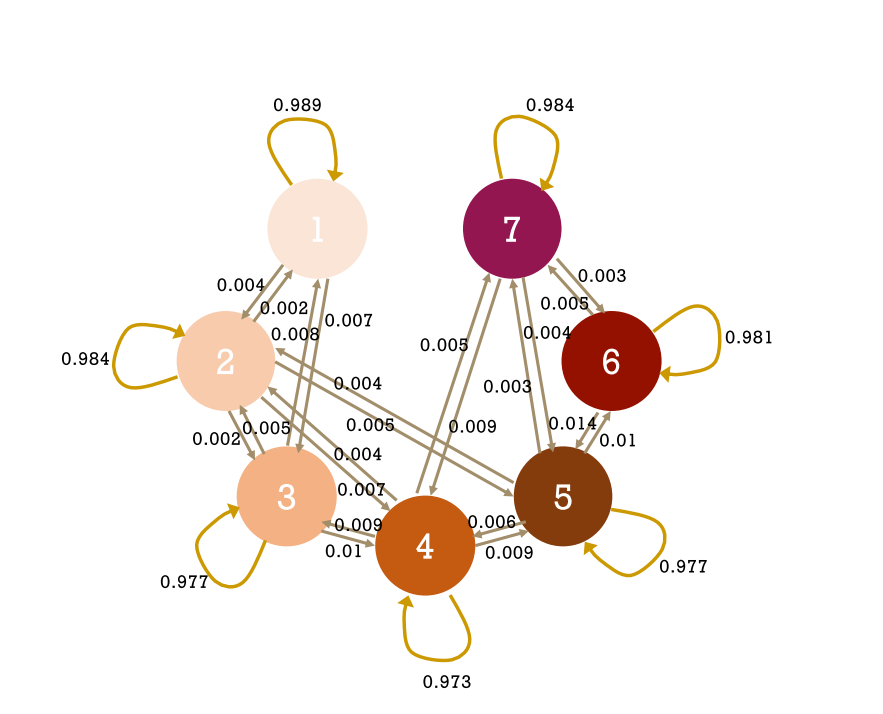
\includegraphics[width=0.5\textwidth]{figures/transitions.png}
       \caption{State transition diagram of the learned HMM.}
   \end{figure}	
   
   For the observations, we collected the number of new cases and deaths for the regions of Munich and Landkreis Munich\footnote{\url{https://github.com/jgehrcke/covid-19-germany-gae}} (where Garching
   is located).
   
   A purely fictional Bavarian king, named Markus IV.,
   rolled his seven-sided die and has it proclaimed that our exam can only take place on-site if the severity
   level in February 2022 is below 6 in Munich and Garching. Will he allow us to conduct the exam in person?
   
   (Note: You do not have to read or understand the referenced paper in order to complete the exercise.)
    
    \textit{For more detailed information, see the provided jupyter notebook \textbf{HMM.ipynb}.}
    
    \subsection*{Package Requirement}
    Make sure you install all the packages which are listed in requirement.txt in your jupyter notebook environment.
    
    
    \subsection*{Passing criteria}
    Detailed information on the passing criteria of this programming exercise are given in the respective jupyter notebooks. 
    
    In short: the exercise is passed if the evaluation on Artemis of both problems is passed.
    
    
    \textbf{A pass will be awarded only if:}
    \vspace{-0.3cm}
    \begin{enumerate}
        \item you submitted the \textbf{correct file} with the \textbf{correct name}.
        \item you \textbf{did not change} the \textbf{variable names} provided by us within the template.
        \item your submitted files can be run in an Anaconda environment (Python 3.7) with the packages provided by the \textit{requirements.txt} \textbf{within a reasonable time (under 5 minutes)}.
        \item like the rest of the programming exercises, this is an individual project and work \textbf{must} be your own. (We will use a plagiarism detection tool and any copied code will annul all bonus exercises from both the copier and the copied person!)
    \end{enumerate}
    
    \begin{thebibliography}{1}
        \bibitem{HMMPaper} Zhou, S., Braca, P., Marano, S., Willett, P., Millefiori, L. M., Gaglione, D., and Pattipati, K. R. (2021). Application of Hidden Markov Models to Analyze, Group and Visualize Spatio-Temporal COVID-19 Data. IEEE Access, 9, 134384-134401.
    \end{thebibliography}
    
    
\end{document}
